%%%---------------------------------------------------------------%%%
%%% Wyzsza Szkola Gospodarki Bachelor's Thesis                    %%%
%%% Prepared by Bruno Axel Kamere                                 %%%
%%% Inspired by Artur M. Brodzki & Piotr Woźniak's WUT template.  %%%
%%% Computer Engineering and Mechatronics Department              %%%
%%% Wyzsza Szkola Gospodarki w Bydgoszczy, 2022                   %%%
%%%---------------------------------------------------------------%%%
% -------------------------------------------------------------------
% 30. INTRODUCTION                                                  %
% -------------------------------------------------------------------


%/-------------------------------- CHAPTER START --------------------------------/%

\chapter{Introduction}
\label{chap:thesis-introduction}

Unmanned aerial vehicles (UAVs) also known as remotely piloted vehicles (RPVs) or Drones, although hardly a new technology, with the first used UAV recorded in history dating back to 1849 \cite{vasileprisacariujdrm2017}, have recently gained a lot of attention from various sectors ranging from entertainment to military. This is going to have an impact that cannot be overseen over the coming years as more and more people find uses of UAVs in various applications. UAVs were initially developed to be used for military operations, mainly surveillance, but they were later armed to also enable them to perform long-distance military operations without putting humans at risk. The United States of America have used these types of UAVs mainly in the wars in the Middle East, where UAVs like the General Atomics MQ-9 Reaper also known as Predator B and Northrop Grumman RQ-4 Global Hawk have been widely deployed \cite{samaanorientxxi2022}.

Despite their use in the military sector, UAVs have also been employed in other sectors such as commercial and entertainment sectors, where UAVs are being used in things like land geography mapping, industrial surveillance, photography and many more. Companies like SZ DJI Technology Co., Ltd. or Shenzhen DJI Sciences and Technologies Ltd. in full, more popularly known as its trade name DJI have had a lot of success in this area, whereas of March 2021 DJI had a 76 percent worldwide market share \cite{djimarketshare2021}. UAVs have also seen great use in the healthcare sector, where companies like Zipline \cite{droneslevy2022} are implementing an end-to-end supply chain system that employs UAVs to supply and deliver medical supplies to hospitals in rural areas in Rwanda that are hard to reach or inefficient to reach by other means of delivery.

Rwanda has also seen great use of UAVs during the COVID-19 pandemic where UAVs were widely used by the Rwanda’s Ministry of Health and the Rwanda National Police to spread COVID-19 awareness in Kigali communities \cite{whoafricarw2020}.

As UAVs gain the market, the need to have robust unmanned aerial systems (UASs) becomes inevitable. Currently, there are not a lot of UASs that are deployed on the cloud. Therefore, in this thesis, a robust, scalable, containerized, highly available unmanned aerial system deployed on the cloud service platform, Amazon Web Services (AWS), solution is proposed, where operators can control UAVs from virtually anywhere in the world through web applications deployed on AWS. The proposed solution consists of a UAV running PX4 operating system together with a Raspberry Pi companion computer with a data-link via MAVLink protocol to a ground control system (GCS), telemetry dashboards and a command-and-control centre application running in a highly available and fault-tolerant AWS cloud infrastructure. The focus of this thesis is to therefore assess the possibilities of implementing such a solution in an efficient, resilient, reliable, and highly available manner and discuss on the pros and cons of the solution.

The proposed solution, as seen in figure \ref{fig:solution-hld-a4}, was developed following the best industry standards in software development and architecture as is going to be described in detail in the next chapters. This thesis is also going to discuss the developments that have already been made in this area as well as areas that need further research and development.

This thesis is divided in 5 chapters; chapter \ref{chap:thesis-introduction} introduces the topic of the thesis, chapter \ref{chap:theory} expands on the concepts, tools and implementation techniques used during development of the proposed solution, chapter \ref{chap:methodology-and-setup} details on how the proposed solution is set up and tested, chapter \ref{chap:discussion} discusses on the implementation of the solution and challenges faced and finally chapter \ref{chap:conclusion} concludes the thesis and discusses on future work on the proposed solution.

\begin{figure}[!htbp]
    \centering 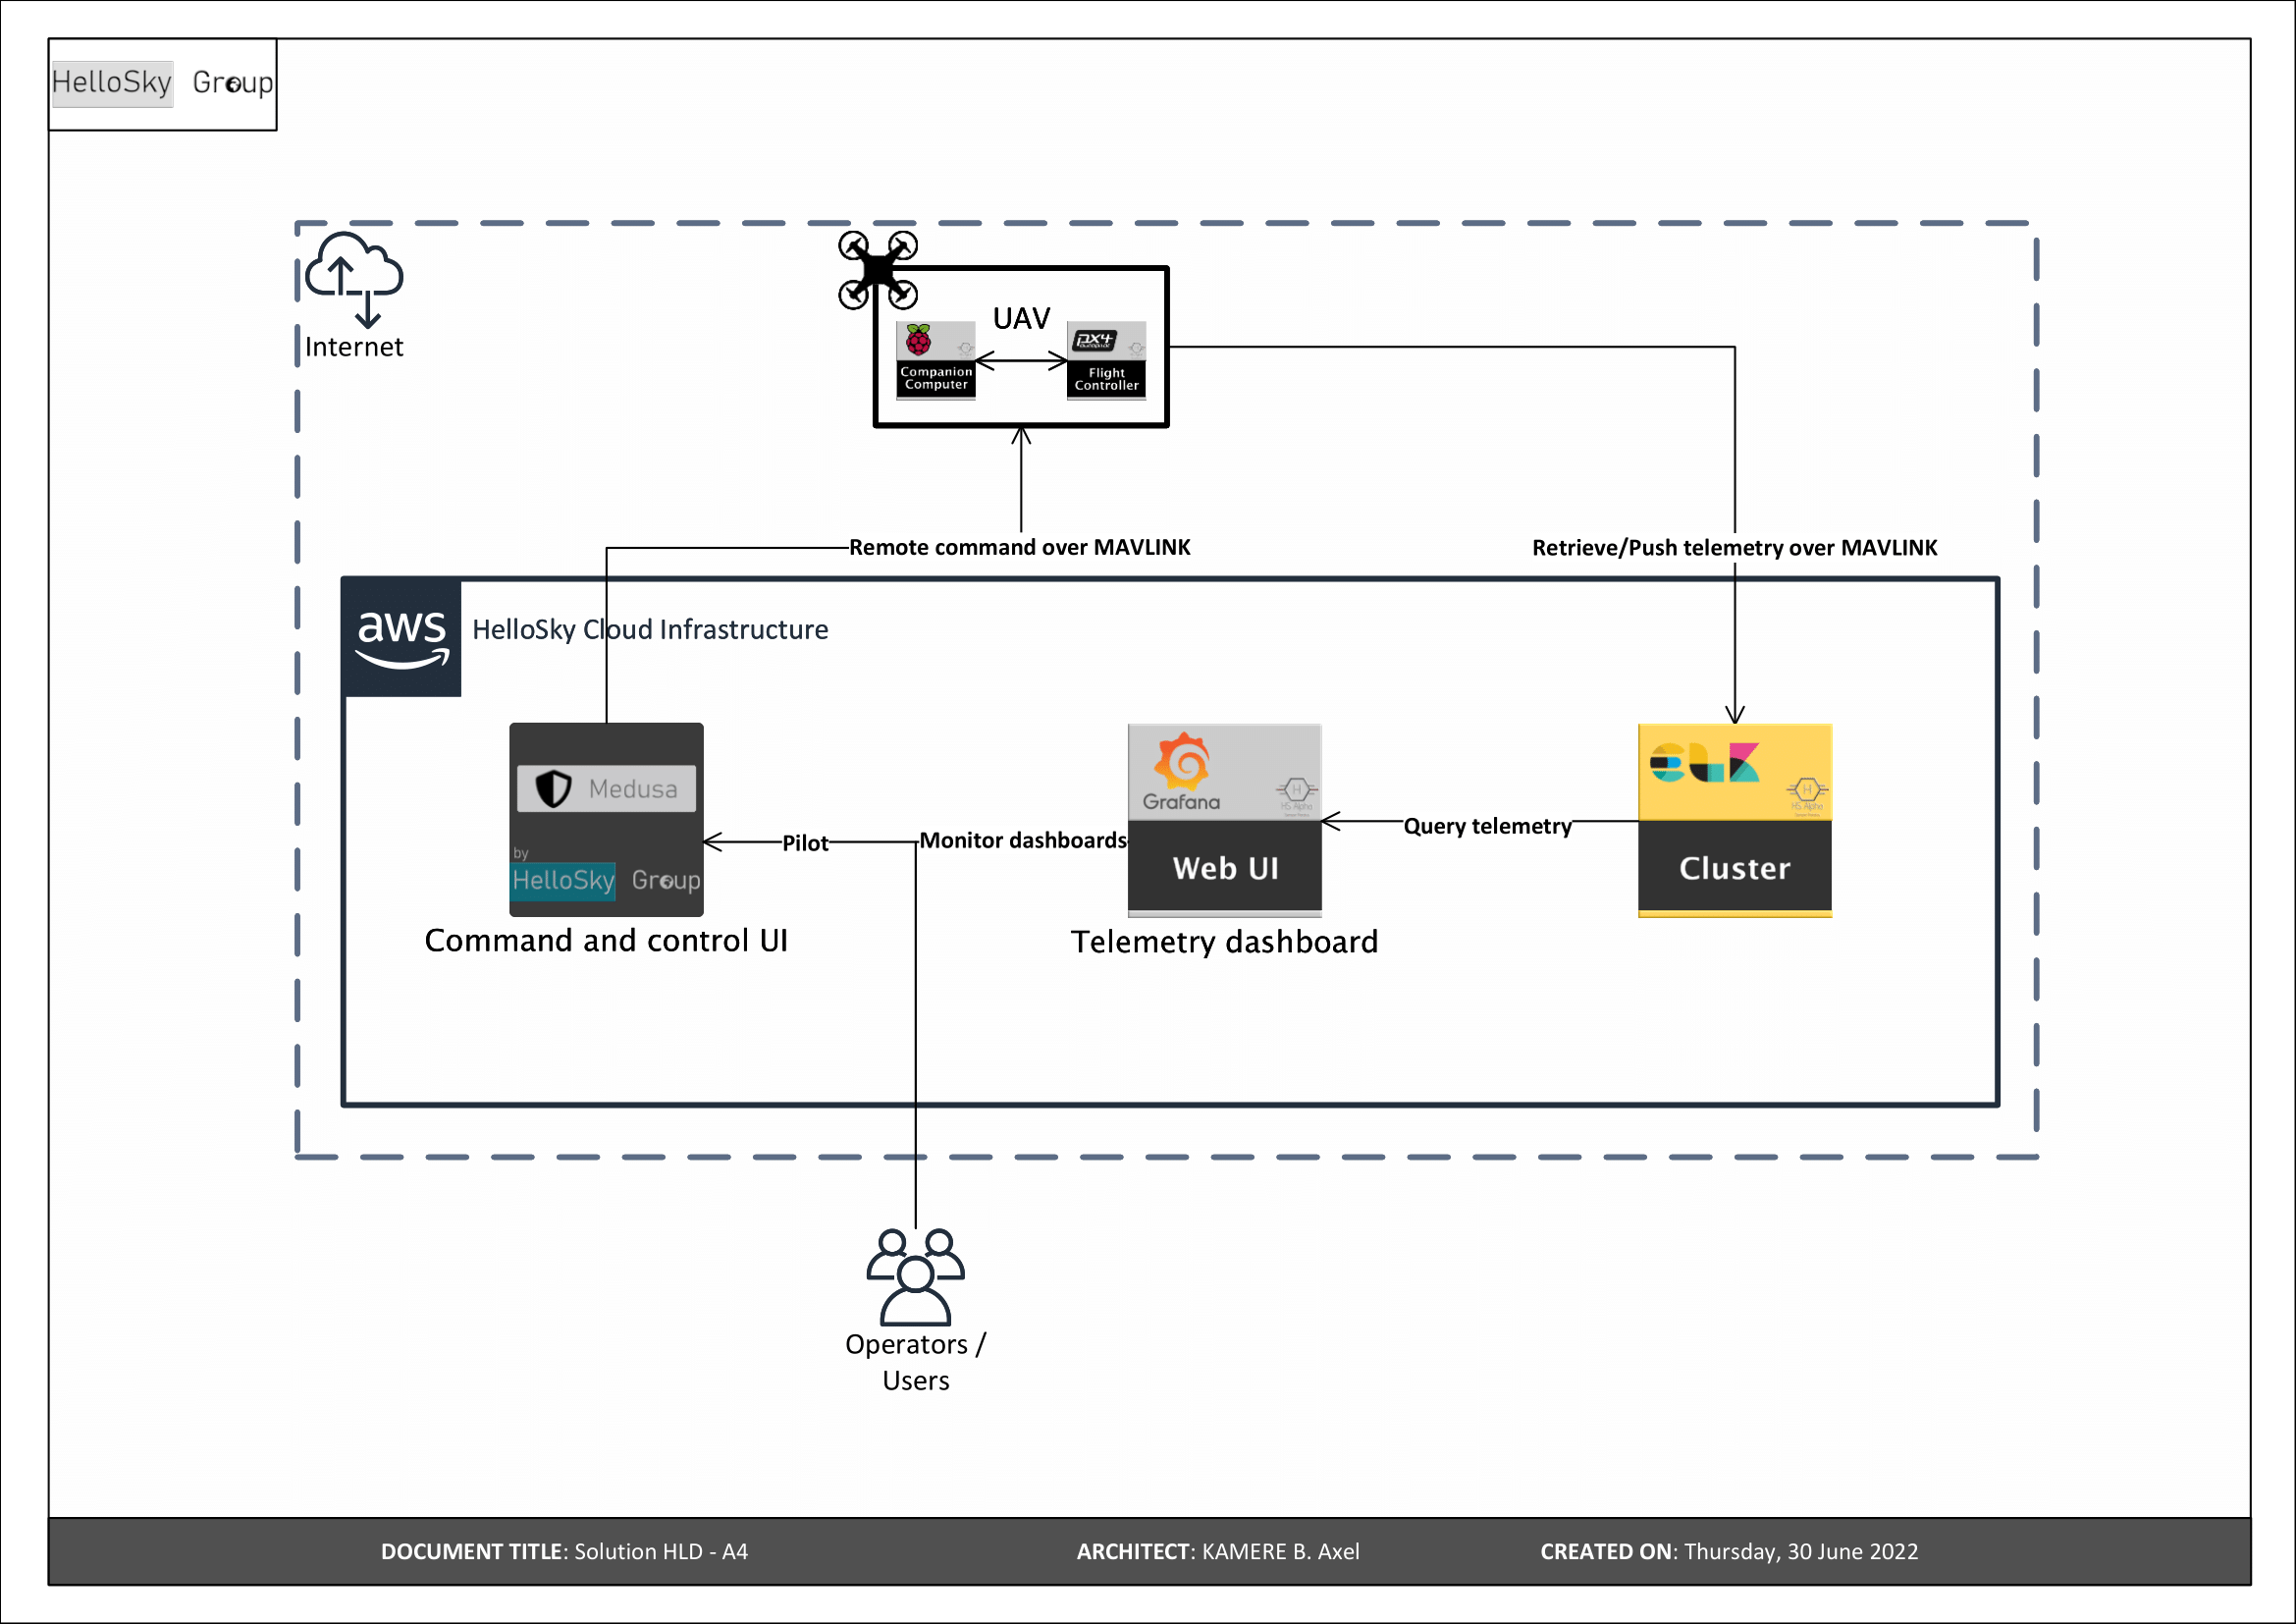
\includegraphics[width=1\linewidth]{solution_hld_a4.png}
    \caption{Proposed solution high-level design.}
    \label{fig:solution-hld-a4}
    \source{Own work. Designed with Affinity Designer. Refer to \ref{subsec:affinity-designer}.}
\end{figure}


%/-------------------------------- SECTION START --------------------------------/%

\section{Related work}
\label{sec:related-work}

UAVs and UASs in general is a field that has undergone substantial development through various researches done by scientists, engineers and academicians.

One of the challenges still faced by UAVs, especially in the capability of being able to deploy them in urban areas, is the safety of their operations. Being able to build a UAV with highly effective collision avoidance algorithms is a still a field under active research. And this is one of the main challenges that need to be solved for the world to see robust autonomous UAVs employed widely in communities for various use cases. Pedro et. al have studied on how UAVs can be made more resilient and safe with the help of artificial intelligence, machine learning and the likes. In their article 'Framework for fully autonomous UAVs' \cite{Pedro2020}, they reviewed the current collision avoidance algorithms for both static and dynamic objects and proposed a conceptual framework to improve more the safety and reliability of UAVs.

In their Master's thesis, Hedström et. Al have also conducted research on "Drones in the Cloud" where they compared several drones IoT architectures and how drones can be simulated in AWS \cite{mscdronesinthecloud}. In their work they compared three different IoT architectures for drones; cloud, fog and edge. They performed measurements to determine which architecture is suited for which type of drone, depending on the drone function. They also did research on how drones can be simulated on AWS to improve development speed and reduce costs during development.

%/--------------------------------- SECTION END ---------------------------------/%


%/-------------------------------- SECTION START --------------------------------/%

\section{Problem definition}
\label{sec:problem-definition}
The cloud technology is an evolving area nowadays due to how agile, efficient, scalable and cost-effective it is to deploy resources on the cloud. Many companies all over the world have seen multiple success stories in using cloud services where, for example, General Electric Renewable Energy has managed to achieve a 99.9\% data availability through its move to the cloud \cite{awsgerenewableenergy}.

The use of cloud services is yet to expand even more to other industries like the aerospace industry, especially in the management of unmanned aerial systems (UAS). As the world sees great use of unmanned aerial vehicles (UAVs), more efficient, reliable, scalable and highly available ways of deploying and operating components of the UAS will need to be developed. Building UASs where the UAV compute power can be on the cloud, as well as other components like the command and control centre would play a big part in advancing the unmanned aerial mobility sector. This can help in increasing the range in which UAVs that rely on battery power operate for example, because the UAV would not need to carry heavy compute power to process its generated data like imagery, as everything would be sent to the cloud to be processed. It would also allow operators to centrally manage a fleet of UAVs from one endpoint instead of having multiple interfaces to manage multiple UAVs.

Therefore, the aim of this thesis is to expand on the research question below:

\begin{itemize}
    \item What advantages does it bring in running applications and UASs on the AWS cloud provider?
\end{itemize}

%/--------------------------------- SECTION END ---------------------------------/%


%/-------------------------------- SECTION START --------------------------------/%

\section{Use case}
\label{sec:use-case}

As UAVs emerge, there will be a need to be able to centrally manage a fleet of UAVs. Depending on the UAV use case, operators might need to also control them at a long distance beyond eyesight. A UAV operates as part of a system comprised of multiple other components that support the operation of a UAV. The main components onboard a UAV are:

\begin{itemize}
    \item Sensors.  For example: distance, IMU, barometer, compass, GPS, \textit{et cetera}.
    \item A battery. To provide power to the UAV.
    \item A flight controller. This is the main component onboard a UAV since it talks directly to the UAV hardware and commands the UAV directly. It runs firmware like PX4 autopilot \cite{px4documentation}.
    \item A companion computer. For more advanced UAV implementations, a companion computer running Linux operating system is added to the system to run onboard computation tasks like collision avoidance algorithms, data-transfer pipelines, \textit{et cetera}. The companion computer communicates with the flight controller via MAVLink, and can also talk out to the internet via LTE/Wi-Fi/Satellite data-link.
    \item A Wi-Fi, LTE or Satellite module. Any of these is needed to help the UAV establish a connection to the ground control station or any other ground API for remote control and mission upload.
\end{itemize}

UAVs can be configured with various payload to fulfil certain missions, below are various UAV use cases:
\begin{itemize}
    \item Agriculture \cite{djienterprisedonesinagriculture}.
    \item Facility inspection \cite{dronesinfacilityinspection}.
    \item Shipping and delivery \cite{insiderintelligence2022}.
    \item Search and rescue \cite{dronesinsearchandrescue}.
    \item Law enforcement \cite{djidronesinlawenforcement}.
    \item Military reconnaissance / Surveillance \cite{dwdronesinbundeswehr}.
\end{itemize}

In any UAV use case, being able to monitor the UAV operation and metrics provided by onboard sensors is key. Therefore, the UAV must have the capability to send telemetry frequently to a ground control station. Metrics transmitted can be:
\begin{itemize}
    \item Ground speed.
    \item Altitude.
    \item Battery levels.
    \item Yaw.
    \item Location.
    \item Direction.
    \item Other data from attached sensors, depending on the UAV use case.
\end{itemize}

With the above metrics and telemetry, a UAV can be made more advanced by implementing fail-safe mechanisms on each of the sensor metrics like:
\begin{itemize}
    \item Taking evasive manoeuvres if on collision course.
    \item What to do if the batteries are low on power.
    \item What to do if out of connectivity range.
\end{itemize}

%/--------------------------------- SECTION END ---------------------------------/%


%/-------------------------------- SECTION START --------------------------------/%

\section{About HelloSky group}
\label{sec:about-hellosky-group}

Across this thesis, there will be mentions of the name "HelloSky group". Several designs built for the project as well as source codes all have mentions of HelloSky group or hsg in abbreviations.

HelloSky group is a name used to label the work done and future developments that will be made on this project and any other related projects that will be built in the future. It is mainly done like so to improve motivation to keep working on the project, be it now or in the future. Figure \ref{fig:hs-group-logos} shows the HelloSky group logos that will be seen across various figures and source codes throughout the thesis project.

\begin{figure}[!htbp]
    \centering
    \begin{subfigure}{0.4\textwidth}
        
\includegraphics[width=\linewidth]{hs_group_wide_500x200.png}
        \caption{Coloured 500 x 200.}
        \label{fig:hs-group-wide-500x200}
    \end{subfigure}
    \hspace*{\fill}
    \begin{subfigure}{0.4\textwidth}
        
\includegraphics[width=\linewidth]{hs_group_wide_dark_500x200.png}
        \caption{Black and white 500 x 200.}
        \label{fig:hs-group-wide-dark-500x200}
    \end{subfigure}
    \caption{HelloSky group logos.}
    \label{fig:hs-group-logos}
    \source{Own work. Designed with Affinity Designer. Refer to \ref{subsec:affinity-designer}.}
\end{figure}

%/--------------------------------- SECTION END ---------------------------------/%

%/--------------------------------- CHAPTER END ---------------------------------/%


%/----------------------------- NOMENCLATURE START ------------------------------/%

\nomenclature[z-UAV]{UAV}{Unmanned Aerial Vehicle}
\nomenclature[z-UAS]{UAS}{Unmanned Aerial System}
\nomenclature[z-GCS]{GCS}{Ground Control Station}
\nomenclature[z-LTE]{LTE}{Long Term Evolution (Telecommunication)}
\nomenclature[z-DJI]{DJI}{Da-Jiang Innovations}
\nomenclature[z-AWS]{AWS}{Amazon Web Services}
\nomenclature[z-HLD]{HLD}{High-Level Design}
\nomenclature[z-HHLD]{HHLD}{High-High-Level Design}
\nomenclature[z-IMU]{IMU}{Inertia Measurement Unit}

%/------------------------------ NOMENCLATURE END -------------------------------/%
